\section{Mesure Psychophysique}
Le sens du toucher peut sentir divers stimuli tactile. Néanmoins, comme tout récepteur/senseur, il ne peut sentir qu’à partir d’une intensité minimum (seuil de perception) et ne peux distinguer qu’une différence minimale entre deux intensités (seuil de discrimination). Ces caractéristiques peuvent être mesuré et quantifié grâce à divers expériences  psychophysiques (exemple tableau ci-dessous).\par
\begin{table}[!h]
	\caption{Seuil de perception (résolution) et seuil de discrimination (weber fraction) pour différent types de sensation (stimulus dimension)}
	\label{tab_mesure_psycho}
	\centering
	\begin{tabular}{|p{5cm}|p{5cm}|p{4cm}|}
		\hline \rule[-7pt]{0pt}{20pt}
		Dimension de la stimulation&Résolution&Fraction de Weber(\%)\\
		\hline
		\rule[-7pt]{0pt}{20pt}Texture de surface (rugosité)& 0.06... & 5-12\% \\
		\hline
		\rule[-7pt]{0pt}{20pt}...&...& ...\\
		\hline
		\rule[-7pt]{0pt}{20pt}...&...&...\\
		\hline 
		\rule[-7pt]{0pt}{20pt}...&...&...\\
		\hline
		\rule[-7pt]{0pt}{20pt}...&...& ...\\
		\hline
		\rule[-7pt]{0pt}{20pt}...&...&...\\
		\hline 
		\rule[-7pt]{0pt}{20pt}...&...&...\\
		\hline
		\rule[-7pt]{0pt}{20pt}...&...& ...\\
		\hline
		\rule[-7pt]{0pt}{20pt}...&...&...\\
		\hline 
		\rule[-7pt]{0pt}{20pt}...&...&...\\
		\hline
		\rule[-7pt]{0pt}{20pt}...&...& ...\\
		\hline
		\rule[-7pt]{0pt}{20pt}...&...&...\\
		\hline 
		\rule[-7pt]{0pt}{20pt}...&...&...\\
		\hline
		\rule[-7pt]{0pt}{20pt}...&...& ...\\
		\hline
		\rule[-7pt]{0pt}{20pt}...&...&...\\
		\hline
	\end{tabular}
\end{table}
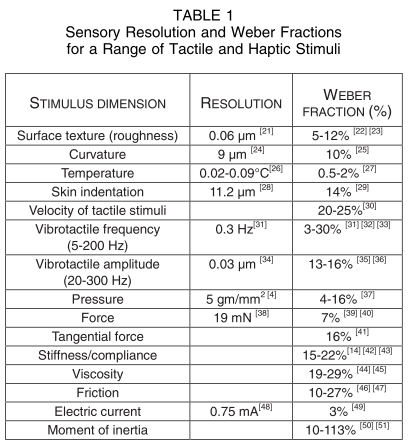
\includegraphics[width=10cm]{1_Bible/Photos/Biology/tab_seuil.png}

\subsection{Seuil de perception -- \textit{Threshold}}
...

\subsection{Seuil de discrimination -- \textit{JND}}
...

\subsubsection{Seuil de discrimination spatiale}
La méthode du seuil de discrimination spatiale consiste à déterminer la distance minimale qu’un sujet (les yeux fermés) n’arrive plus à distinguer les deux pointes qui lui appliqué sur la peau. En fonction des différentes partie du corps, le seuil – entre ressentir les deux pointes et le passage ou le sujet ne pense qu’il n’y en a plus qu’une. Zones plus sensible de que d’autre. Les MRs ne sont pas réparti de la façon sur le corps, la densité est différente.\par
\begin{figure}[!h]
	\centering
	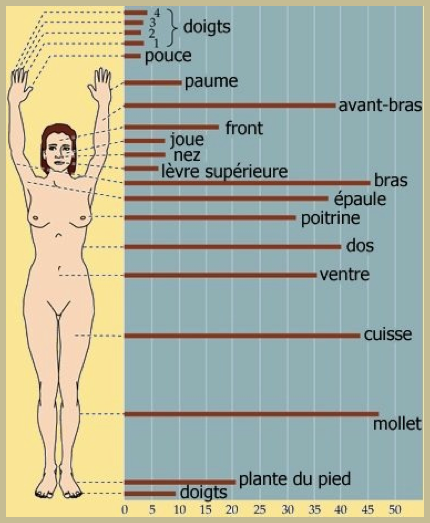
\includegraphics[width=10cm]{1_Bible/Photos/Biology/discrim_spatiale.png}
	\caption{Tests des deux points}\label{discrim_spatiale}
\end{figure}
Les parties les plus sensibles sont les mains, le visage et les doigts de pieds.

\subsection{Méthode de mesures psychophysique}
...

\subsubsection{Méthode classique}
...

\subsubsection{Théorie de la détection du signal}
...




